\documentclass[a4paper, 12pt]{article}
\usepackage[a4paper,top=1.5cm, bottom=1.5cm, left=1cm, right=1cm]{geometry}
\usepackage[utf8]{inputenc}
\usepackage{mathtext}
\usepackage{amsmath}
\usepackage{amsfonts}
\usepackage[english, russian]{babel}
\usepackage{indentfirst}
\usepackage{longtable}
\usepackage{graphicx}
\graphicspath{{pictures/}}
\DeclareGraphicsExtensions{.pdf,.png,.jpg}
\usepackage{natbib}
\usepackage{hyperref}
\usepackage{emoji}
\babelfont{rm}{Droid Serif}
\babelfont{sf}{Droid Sans}
\renewcommand{\baselinestretch}{1.3}
\usepackage{wrapfig}

\author{Платонов Егор Б04-301}
\title{1.2.3 Определение моментов инерции твердых тел с помощью трифилярного подвеса}
\date{}
\begin{document}
\maketitle
\section*{Теоретические сведения}
Момент инерции твердого тела рассчитывается по формуле:
\begin{equation}
I = \int r^2dm
\end{equation}
Далеко не всегда удается вычислить момент инерции тела аналитически ввиду неоднородности или сложной формы, в таких случаях удобно сделать это экспериментально, например, с помощью трифилярного подвеса.
\begin{figure}[h!]
\begin{center}
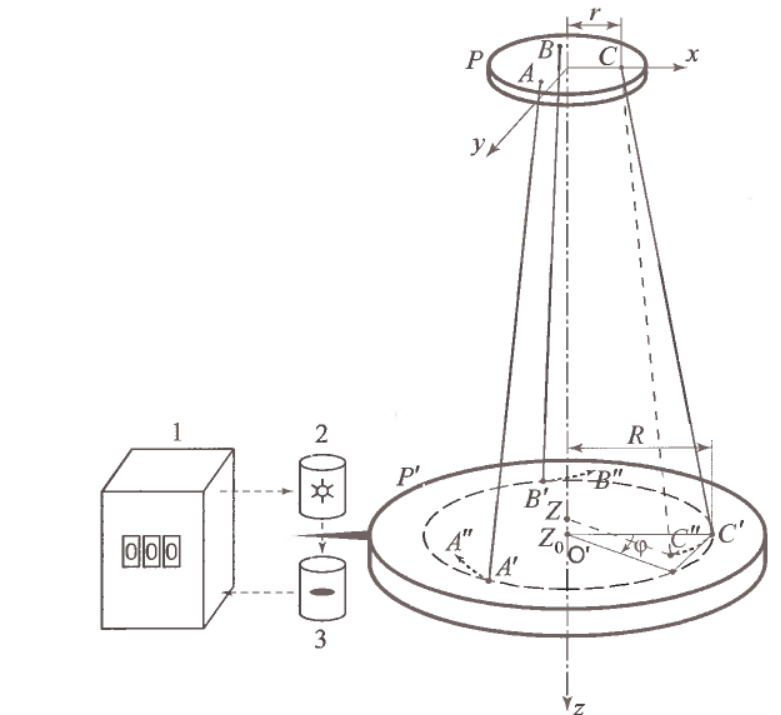
\includegraphics[width=0.7\textwidth]{Подвес}
\end{center}
\caption{Трифилярный подвес} \label{подвес}
\end{figure}
Устройство состоит из неподвижной платформы, вращающейся платформы, подвешенной на трех симметричных нитях.
Если пренебречь потерями энергии, то уравнение сохранения энергии при колебания:
\begin{equation}
\label{энергия}
\frac{I\dot{\varphi}^2}{2}+mg(z_0-z)=E,
\end{equation}
где $I$ - момент инерции платформы и тела, $z_0$ - координата по вертикали центра нижней платформы при равновесии, $z$ - координата аналогичной точки при повороте на угол $\phi$.
Из уравнения \ref{энергия} видно, что колебательное движение системы происходит благодаря силе тяжести. 

Рассмторим точку C на верхней платформе с координатами $(r, 0, 0)$ и точку $C''$, противоположную С при повороте на $\phi$, с координатами $(R\cos(\varphi), R\sin(\varphi)), z)$
Расстояние между нимим равно длине нити:
\begin{equation}
(R\cos(\phi)-r)^2+R^2\sin^2\phi+z^2=L^2
\end{equation}
Для малых углов:
\begin{equation}
z^2=L^2-R^2-r^2+2Rr\cos\varphi=z_0^2-2Rr(1-\cos\varphi)\approx z_0^2-Rr\varphi^2
\end{equation}
\begin{equation}
z \approx \sqrt{z_0^2-Rr\varphi^2}\approx z_0 \sqrt{1-\frac{Rr\varphi^2}{z_0^2}} \approx z_0- \frac{Rr\varphi^2}{2z_0}
\end{equation}
Подставив это в уравнение \ref{энергия}:
\begin{equation}
\frac{1}{2}I\dot{\varphi}+mg\frac{Rr}{2z_0}\varphi^2=E
\end{equation}
Откуда:
\begin{equation}
\varphi=\varphi_0\sin(\sqrt{\frac{mgRr}{Iz_0}}t+\Theta)
\end{equation}
Константны определяются начальными условиями, а период колебаний системы:
\begin{equation}
T=2\pi\sqrt{\frac{Iz_0}{mgRr}}
\end{equation}
Откуда не трудно определить выражние для момента инерции:
\begin{equation}
I=\frac{mgRrT^2}{4\pi^2z_0}
\end{equation}
Для краткости:
\begin{equation}
I=kmT^2
\end{equation}
Для постоянной k для данной установки:
\begin{equation}
k=\frac{gRr}{4\pi^2z_0}
\end{equation}

\section*{Измерения параметров установки}
\newpage
\begin{table}[ht]
\label{геом}
\caption{Параметры установки}
\centering
\begin{tabular}{|c|c|c|c|c|c|c|}
\hline $z_0$, м& $R$, мм & r, мм & $m_0$, г & k $ \cdot 10^{4} \text{, м}^2/\text{c}^2$ & $\sigma_k \cdot 10^{4}$, $\text{м}^2/\text{c}^2$ & $\varepsilon_k$, $\%$\\ 
\hline $2,148 \pm 0,001$ & $115,4 \pm 0,5$ & $30,5 \pm 0,3$ & $993,5 \pm 0,5$ & $4,07$ & $0,044$ & $1,08$ \\ 
\hline 
\end{tabular} 
\end{table}
$\varepsilon_{z_0} = 0,046\%$, $\varepsilon_R = 0,433\%$, $\varepsilon_r = 0,984\%$
\[ \varepsilon_k = \sqrt{\varepsilon_{z_0}^2+\varepsilon_R^2+\varepsilon_r^2}\]

\section*{Измерение моментов инерции различных тел}

\begin{table}[!ht]
    \centering
    \begin{tabular}{|l|l|l|l|}
    \hline
        тело & диск & паралеллепипед & кольцо \\ \hline
        $m$, г & $580,3 \pm 0,1$ & $1101 \pm 0,1$ & $737,3 \pm 0,1$ \\ \hline
    \end{tabular}
    \caption{Массы тел}
\end{table}

Далее были проведены измерения периодов 5 колебаний установки (с нагрузкой и без). $T = \frac{t}{5}$. Для пустой платформы приведены формулы расчета погрешностей и систематическая погрешность периода. Для остальных случаев используются такие же формулы и такая же систематическая погрешность.

\subsection*{Пустая платформа}

\begin{wraptable}{r}{8cm}
    \centering
    \begin{tabular}{|l|l|}
    \hline
        t, с & T, с \\ \hline
        22,166 & 4,4332 \\ \hline
        22,213 & 4,4426 \\ \hline
        22,208 & 4,4416 \\ \hline
        22,211 & 4,4422 \\ \hline
        22,193 & 4,4386 \\ \hline
    \end{tabular}
    \caption{Измерения периода колебаний пустой платформы}
\end{wraptable}

\[ \langle T \rangle = 4,44 \text{ c}\]

\[ \sigma_T^{\text{сист}} = 0,001 \text{ c}\]

\[ \sigma_T^{\text{случ}} = \sqrt{\frac{\sum_{i=1}^{N}(T_i-\langle T \rangle)^2}{N(N-1)}} = 0,0018 \text{ c}\]

\[ \sigma_T^{\text{полн}} = \sqrt{\sigma_T^{{\text{сист}}^2}+\sigma_T^{{\text{случ}}^2}} = 0,002 \text{ c}\]

\[ \varepsilon_T = \frac{\sigma_T^{\text{полн}}}{\langle T \rangle} = 0,045\%\]

\[\varepsilon_{m_0} = \frac{0,5}{993,5} \cdot 100 = 0,05\%\]

\[ I_0 = km_0 {\langle T \rangle}^2 = 7,97 \text{ г}\cdot\text{м}^2\]

\[ \varepsilon_{I_0} = \sqrt{\varepsilon_{m_0}^2 + 4\varepsilon_T^2 + \varepsilon_k} = 1,085\%\]

\subsection*{Диск}

\begin{wraptable}{r}{6cm}
    \centering
    \begin{tabular}{|l|l|}
    \hline
        t, с & T, с \\ \hline
        19,854 & 3,9708 \\ \hline
        19,856 & 3,9712 \\ \hline
        19,844 & 3,9688 \\ \hline
        19,851 & 3,9702 \\ \hline
        19,852 & 3,9704 \\ \hline
    \end{tabular}
    \caption{Измерения периода колебаний диска на платформе}
\end{wraptable}

\[ \langle T \rangle = 3,97 \text{ c}\]

\[\sigma_T^{\text{случ}} = 0,0004 \text{ c}\]

\[\sigma_T^{\text{полн}} = 0,0011 \text{ с}\]

\[\varepsilon_T = 0,027\% \]

\[\varepsilon_{m_0+m_\text{д}} = \frac{0,5+0,1}{993,5+580,3} \cdot 100 = 0,038\%\]

\[ I_{0+\text{д}} = k(m_0+m_\text{д}) {\langle T \rangle}^2 = 10,097 \text{ г}\cdot\text{м}^2\]

\[ \varepsilon_{I_{0+\text{д}}} = \sqrt{\varepsilon_{m_0+m_\text{д}}^2 + 4\varepsilon_T^2 + \varepsilon_k} = 1,082\%\]

\[ I_\text{д} = I_{0+\text{д}} - I_0 = 2,127 \text{ г}\cdot\text{м}^2\]

\[ \sigma_{I_\text{д}} = I_{0+\text{д}}\varepsilon_{I_{0+\text{д}}} + I_0\varepsilon_{I_0} = 0,196 \text{ г}\cdot\text{м}^2 (\varepsilon_{I_\text{д}} = 9,2\%) \]

\subsection*{Паралеллепипед (в горизонтальном положении)}

\begin{wraptable}{r}{6cm}
    \centering
    \begin{tabular}{|l|l|}
    \hline
        t, с & T, с \\ \hline
        19,043 & 3,8086 \\ \hline
        19,008 & 3,8016 \\ \hline
        18,999 & 3,7998 \\ \hline
        19,002 & 3,8004 \\ \hline
        18,989 & 3,7978 \\ \hline
    \end{tabular}
    \caption{Измерения периода колебаний паралеллепипеда (в горизонтальном положении) на платформе}
\end{wraptable}

\[ \langle T \rangle = 3,8 \text{ c}\]

\[\sigma_T^{\text{случ}} = 0,0018 \text{ c}\]

\[\sigma_T^{\text{полн}} = 0,0021 \text{ с}\]

\[\varepsilon_T = 0,055\% \]

\[\varepsilon_{m_0+m_\text{п}} = \frac{0,5+0,1}{993,5+1101} \cdot 100 = 0,029\%\]

\[ I_{0+\text{пг}} = k(m_0+m_\text{п}) {\langle T \rangle}^2 = 12,32 \text{ г}\cdot\text{м}^2\]

\[ \varepsilon_{I_{0+\text{пг}}} = \sqrt{\varepsilon_{m_0+m_\text{п}}^2 + 4\varepsilon_T^2 + \varepsilon_k} = 1,08\%\]

\[ I_\text{пг} = I_{0+\text{пг}} - I_0 = 4,35 \text{ г}\cdot\text{м}^2\]

\[ \sigma_{I_\text{пг}} = I_{0+\text{пг}}\varepsilon_{I_{0+\text{пг}}} + I_0\varepsilon_{I_0} = 0,219 \text{ г}\cdot\text{м}^2 (\varepsilon_{I_\text{пг}} = 5\%) \]

\subsection*{Паралеллепипед (в вертикальном положении)}

\begin{wraptable}{r}{8cm}
    \centering
    \begin{tabular}{|l|l|}
    \hline
        t, с & T, с \\ \hline
        15,571 & 3,1142 \\ \hline
        15,556 & 3,1112 \\ \hline
        15,539 & 3,1078 \\ \hline
        15,538 & 3,1076 \\ \hline
        15,516 & 3,1032 \\ \hline
    \end{tabular}
    \caption{Измерения периода колебаний паралеллепипеда (в вертикальном положении) на платформе}
\end{wraptable}

\[ \langle T \rangle = 3,12 \text{ c}\]

\[\sigma_T^{\text{случ}} = 0,00185 \text{ c}\]

\[\sigma_T^{\text{полн}} = 0,00211 \text{ с}\]

\[\varepsilon_T = 0,068\% \]

\[\varepsilon_{m_0+m_\text{п}} = \frac{0,5+0,1}{993,5+1101} \cdot 100 = 0,029\%\]

\[ I_{0+\text{пв}} = k(m_0+m_\text{п}) {\langle T \rangle}^2 = 8,239 \text{ г}\cdot\text{м}^2\]

\[ \varepsilon_{I_{0+\text{пв}}} = \sqrt{\varepsilon_{m_0+m_\text{п}}^2 + 4\varepsilon_T^2 + \varepsilon_k} = 1,089\%\]

\[ I_\text{пв} = I_{0+\text{пв}} - I_0 = 0,269 \text{ г}\cdot\text{м}^2\]

\[ \sigma_{I_\text{пв}} = I_{0+\text{пв}}\varepsilon_{I_{0+\text{пв}}} + I_0\varepsilon_{I_0} = 0,176 \text{ г}\cdot\text{м}^2 (\varepsilon_{I_\text{пв}} = 65,5\%) \]

\subsection*{Кольцо}

\begin{wraptable}{r}{8cm}
    \centering
    \begin{tabular}{|l|l|}
    \hline
        t, с & T, с \\ \hline
        21,512 & 4,3024 \\ \hline
        21,543 & 4,3086 \\ \hline
        21,469 & 4,2938 \\ \hline
        21,508 & 4,3016 \\ \hline
        21,454 & 4,2908 \\ \hline
    \end{tabular}
    \caption{Измерения периода колебаний кольца на платформе}
\end{wraptable}

\[ \langle T \rangle = 4,3 \text{ c}\]

\[\sigma_T^{\text{случ}} = 0,0032 \text{ c}\]

\[\sigma_T^{\text{полн}} = 0,0033 \text{ с}\]

\[\varepsilon_T = 0,078\% \]

\[\varepsilon_{m_0+m_\text{к}} = \frac{0,5+0,1}{993,5+737,4} \cdot 100 = 0,035\%\]

\[ I_{0+\text{к}} = k(m_0+m_\text{к}) {\langle T \rangle}^2 = 13,022 \text{ г}\cdot\text{м}^2\]

\[ \varepsilon_{I_{0+\text{к}}} = \sqrt{\varepsilon_{m_0+m_\text{к}}^2 + 4\varepsilon_T^2 + \varepsilon_k} = 1,092\%\]

\[ I_\text{к} = I_{0+\text{к}} - I_0 = 5,052 \text{ г}\cdot\text{м}^2\]

\[ \sigma_{I_\text{к}} = I_{0+\text{к}}\varepsilon_{I_{0+\text{к}}} + I_0\varepsilon_{I_0} = 0,229 \text{ г}\cdot\text{м}^2 (\varepsilon_{I_\text{д}} = 4,5\%) \]

\subsection*{Кольцо и диск}

\begin{wraptable}{r}{6cm}
    \centering
    \begin{tabular}{|l|l|}
    \hline
        t, с & T, с \\ \hline
        20,079 & 4,0158 \\ \hline
        20,081 & 4,0162 \\ \hline
        20,018 & 4,0036 \\ \hline
        20,005 & 4,001 \\ \hline
        20,017 & 4,0034 \\ \hline
    \end{tabular}
    \caption{Измерения периода колебаний кольца и диска на платформе}
\end{wraptable}

\[ \langle T \rangle = 4,01 \text{ c}\]

\[\sigma_T^{\text{случ}} = 0,0032 \text{ c}\]

\[\sigma_T^{\text{полн}} = 0,00345 \text{ с}\]

\[\varepsilon_T = 0,086\% \]

\[\varepsilon_{m_0+m_\text{д}+m_\text{к}} = \frac{0,5+0,1+0,1}{993,5+580,3+737,4} \cdot 100 = 0,03\%\]

\[ I_{0+\text{д}+\text{к}} = k(m_0+m_\text{д}+m_\text{к}) {\langle T \rangle}^2 = 15,111 \text{ г}\cdot\text{м}^2\]

\[ \varepsilon_{I_{0+\text{д}+\text{к}}} = \sqrt{\varepsilon_{m_0+m_\text{д}+m_\text{к}}^2 + 4\varepsilon_T^2 + \varepsilon_k} = 1,094\%\]

\[ I_{\text{д}+\text{к}} = I_{0+\text{д}+\text{к}} - I_0 = 7,141 \text{ г}\cdot\text{м}^2\]

\[ \sigma_{I_{\text{к}+\text{д}}} = I_{0+\text{д}+\text{к}}\varepsilon_{I_{0+\text{д}+\text{к}}} + I_0\varepsilon_{I_0} = 0,252 \text{ г}\cdot\text{м}^2 (\varepsilon_{I_{\text{к}+\text{д}}} = 3,5\%) \]

\subsection*{Паралеллепипед (в вертикальном положении) и кольцо}

\begin{wraptable}{r}{8cm}
    \centering
    \begin{tabular}{|l|l|}
    \hline
        t, с & T, с \\ \hline
        17,095 & 3,419 \\ \hline
        17,042 & 3,4084 \\ \hline
        16,953 & 3,3906 \\ \hline
        16,999 & 3,3998 \\ \hline
        17,005 & 3,401 \\ \hline
    \end{tabular}
    \caption{Измерения периода колебаний паралеллепипеда (в вертикальном положении) и кольца на платформе}
\end{wraptable}
.

\[ \langle T \rangle = 3,4 \text{ c}\]

\[\sigma_T^{\text{случ}} = 0,0047 \text{ c}\]

\[\sigma_T^{\text{полн}} = 0,00485 \text{ с}\]

\[\varepsilon_T = 0,142\% \]

\[\varepsilon_{m_0+m_\text{п}+m_\text{к}} = \frac{0,5+0,1+0,1}{993,5+1101+737,4} \cdot 100 = 0,025\%\]

\[ I_{0+\text{пв}+\text{к}} = k(m_0+m_\text{п}+m_\text{к}) {\langle T \rangle}^2 = 13,353 \text{ г}\cdot\text{м}^2\]

\[ \varepsilon_{I_{0+\text{пв}+\text{к}}} = \sqrt{\varepsilon_{m_0+m_\text{п}+m_\text{к}}^2 + 4\varepsilon_T^2 + \varepsilon_k} = 1,117\%\]

\[ I_{\text{пв}+\text{к}} = I_{0+\text{пв}+\text{к}} - I_0 = 5,383 \text{ г}\cdot\text{м}^2\]

\[ \sigma_{I_{\text{пв}+\text{к}}} = I_{0+\text{пв}+\text{к}}\varepsilon_{I_{0+\text{пв}+\text{к}}} + I_0\varepsilon_{I_0} = 0,236 \text{ г}\cdot\text{м}^2 (\varepsilon_{I_{\text{пв}+\text{к}}} = 4,4\%) \]

\section*{Результаты измерений моментов инерции различных тел}
Для проверки правильности метода были выбраны тела момент инерции которых несложно вычислить из их геометрических характеристик.

\begin{table}[!ht]
    \centering
    \begin{tabular}{|l|l|l|l|l|}
    \hline
         & диск & паралеллепипед(гор) & паралеллепипед(верт) & кольцо \\ \hline
        $I_\text{эксп}$, $\text{ г}\cdot\text{м}^2$ & 2,127 & 4,35 & 0,269 & 5,052 \\ \hline
        $I_\text{геом}$, $\text{ г}\cdot\text{м}^2$ & 2,096 & 4,1 & 0,115 & 4,84 \\ \hline
    \end{tabular}
    \caption{Сравнение экспериментально полученных моментов инерции ($I_\text{эксп}$) с моментами инерции вычисленными по геометрическим характеристикам ($I_\text{геом}$})
\end{table}

\section*{Проверка аддитивности моментов инерции}

$I_{0+\text{д}+\text{к}} = 7,141 \text{ г}\cdot\text{м}^2$, $I_\text{д}+I_\text{к} = 7,179 \text{ г}\cdot\text{м}^2 (\Delta I = 0,038 \text{ г}\cdot\text{м}^2)$

$I_{0+\text{пв}+\text{к}} = 5,383 \text{ г}\cdot\text{м}^2$, $I_\text{пв}+I_\text{к} = 5,321 \text{ г}\cdot\text{м}^2 (\Delta I = 0,062 \text{ г}\cdot\text{м}^2)$

\section*{Момент инерции половинок}

Масса половинки диска: 763,95 г.

\begin{table}[!ht]
    \centering
    \begin{tabular}{|l|l|l|l|l|l|}
    \hline
        $h$, см & $t_1$, с & $t_2$, с & $t_3$, с & $T$, с & $I$, г$\cdot$м$^2$ \\ \hline
        0 & 15,371 & 15,342 & 15,343 & 3,0704 & 9,674445279 \\ \hline
        0,5 & 15,451 & 15,443 & 15,401 & 3,086333333 & 9,775113674 \\ \hline
        1 & 15,536 & 15,508 & 15,49 & 3,102266667 & 9,876303119 \\ \hline
        1,5 & 15,667 & 15,718 & 15,725 & 3,140666667 & 10,122315 \\ \hline
        2 & 15,896 & 15,917 & 15,893 & 3,1804 & 10,38005482 \\ \hline
        2,5 & 16,149 & 16,132 & 16,088 & 3,2246 & 10,67057584 \\ \hline
        3 & 16,845 & 16,799 & 16,71 & 3,356933333 & 11,56435968 \\ \hline
    \end{tabular}
    \caption{Зависимость момента инерции половинок диска ($I$) от расстояния между осью вращения и их центрами ($h$)}
\end{table}

\begin{figure}[h]
    \centering
    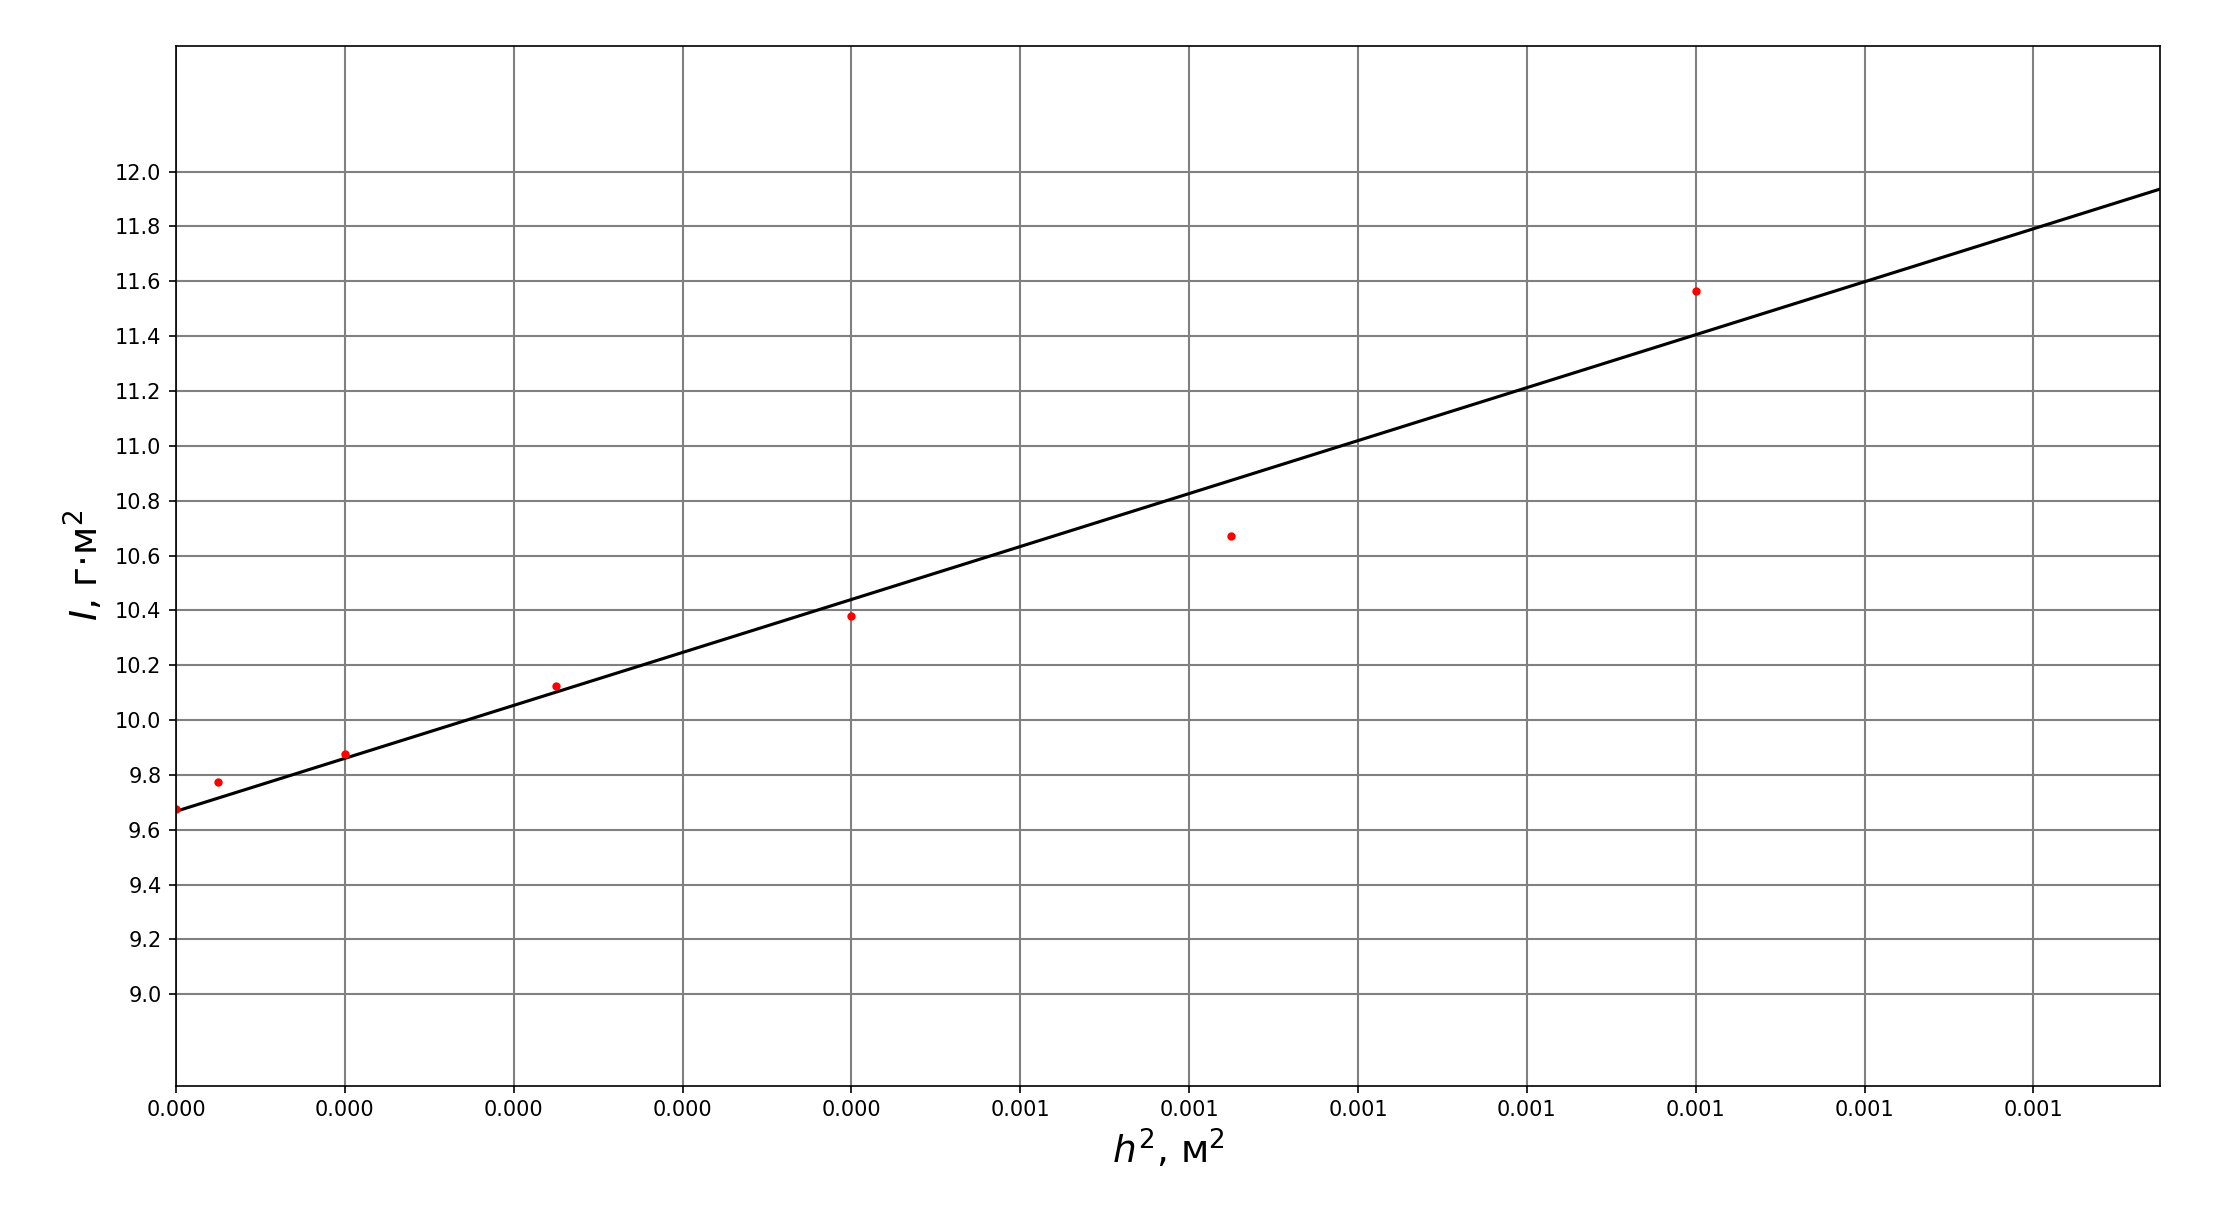
\includegraphics[scale=0.5]{Screenshot 2023-11-29 134502.png}
    \caption{Зависимость $I(h^2)$}
    \label{fig:enter-label}
\end{figure}

Коэффициент наклона $k_1$ равен 1931 г. Ось ординат график пересекает в значении 9,67 $\text{ г}\cdot\text{м}^2$. Согласно теореме Гюйгенса-Штейнера коэффициентом наклона должна быть масса диска, а значение в 0 должно быть равно моменту инерции диска (+момент инерции пустой платформы). $I_\text{диск} = 9,67-7,97 = 1,7 \text{ г}\cdot\text{м}^2$

\[ \sigma_k = 147,87 г\]
\[ \varepsilon_k = 7,6 \%\]
Момент инерции диска был посчитан по его геометрическим параметрам, он равен $1,48 \text{ г}\cdot\text{м}^2$, полученное из графика значение отличается на 13 \%, полученное значение массы отличается от измеренного весами на 21 \%.

\section*{Вывод}
В ходе работы были определены моменты инерции различных фигур с помощью трифилярного подвеса, полученные результаты соответствуют измеренными. Также была проверена экспериментально аддитивность моментов инерции. Также (но в пределах большой погрешности) была подтверждена теорема Гюйгенса-Штейнера.
\end{document}